% ******************************* Thesis Appendix A ********************************
\chapter{Source Implementation in VHDL} 
\label{appendix:1}
%The following source Codes in this Appendix A shows the implementation of
%the Invariant Observer. 
%The Source Codes are written in VHDL 1993 and shows a description about the Behavioural Specification
%of the design. \newline \newline
%Observer.vhd is the entity specification of an Observer Stage and shows specifications about the input and outputs. 
%Figure~\ref{fig:observerstages} shows us an excerpt of the input and output but at most how the several observer stages interact together.
%&\newline
%Observer\_behave.vhd describes the exact behaviour of an observer stage. A detailed description of this behaviour is shown in  Chapter~\ref{chapter:sub:2}.
%\lstinputlisting[language=VHDL]{../../../../vhdl/Observer.vhd}
\begin{comment}
%\phantomsection\addcontentsline{toc}{figure}{Entity Design of Invariant Observer}
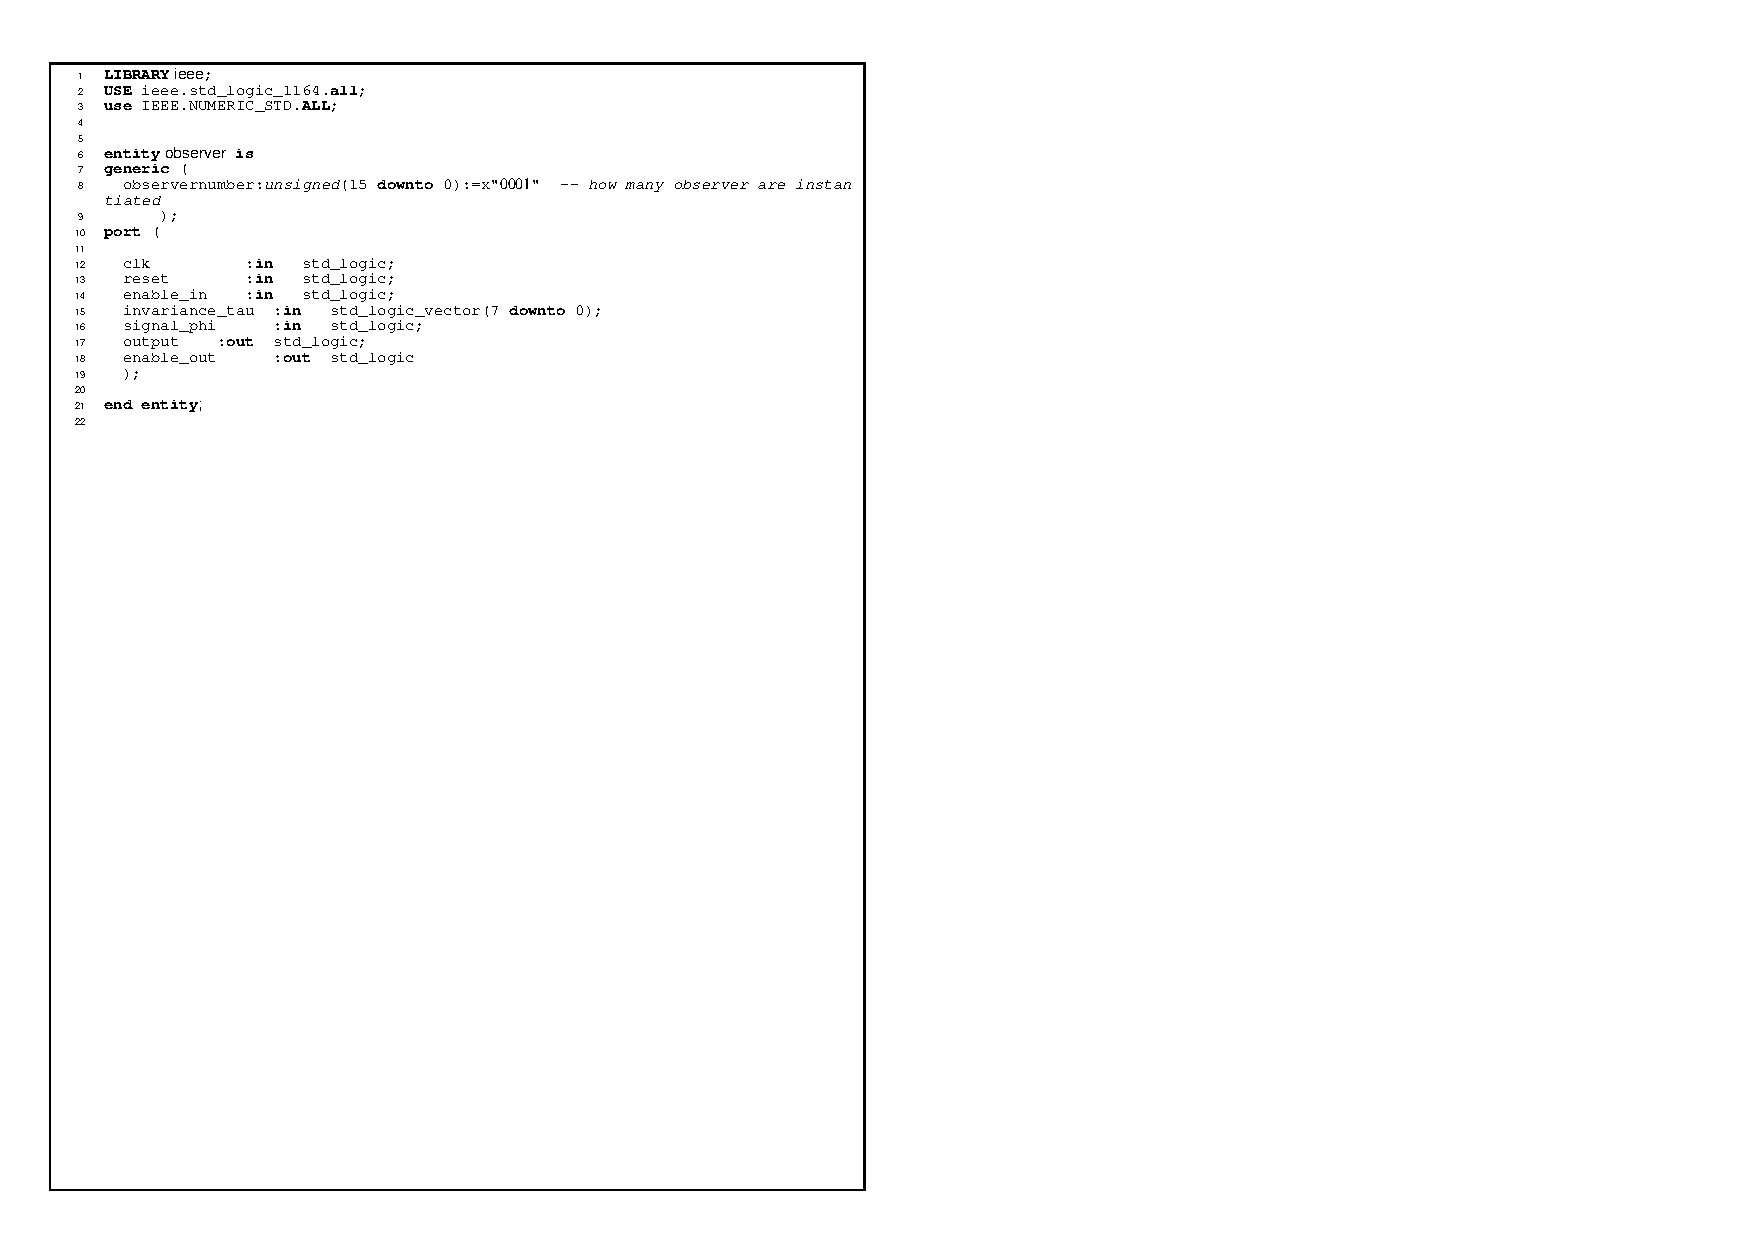
\includepdf[
 pages={-},
 nup=1x1,
 %landscape=false,
 %fitpaper=true,
 %noautoscale=false,
 turn=false,
 scale=1.5, 
 %trim= 0mm 0mm 0mm 0mm,
 clip=true,
 %pagecommand={\label{appendix:source:1}},
 pagecommand={},
 %delta=0mm 0mm
 offset=-80mm 10mm,
 %addtotoc={1,figure,1,{Entity Design of Invariant Observer},{appendix:source:1}}
]{Appendix1/pdf/Observer_2.pdf}
%\caption[Entity Design of Invariant Observer]{Code of Observer Entity Design}
%\label{appendix:source:1}


%\phantomsection\addcontentsline{toc}{figure}{Behavioural Design of Invariant Observer}
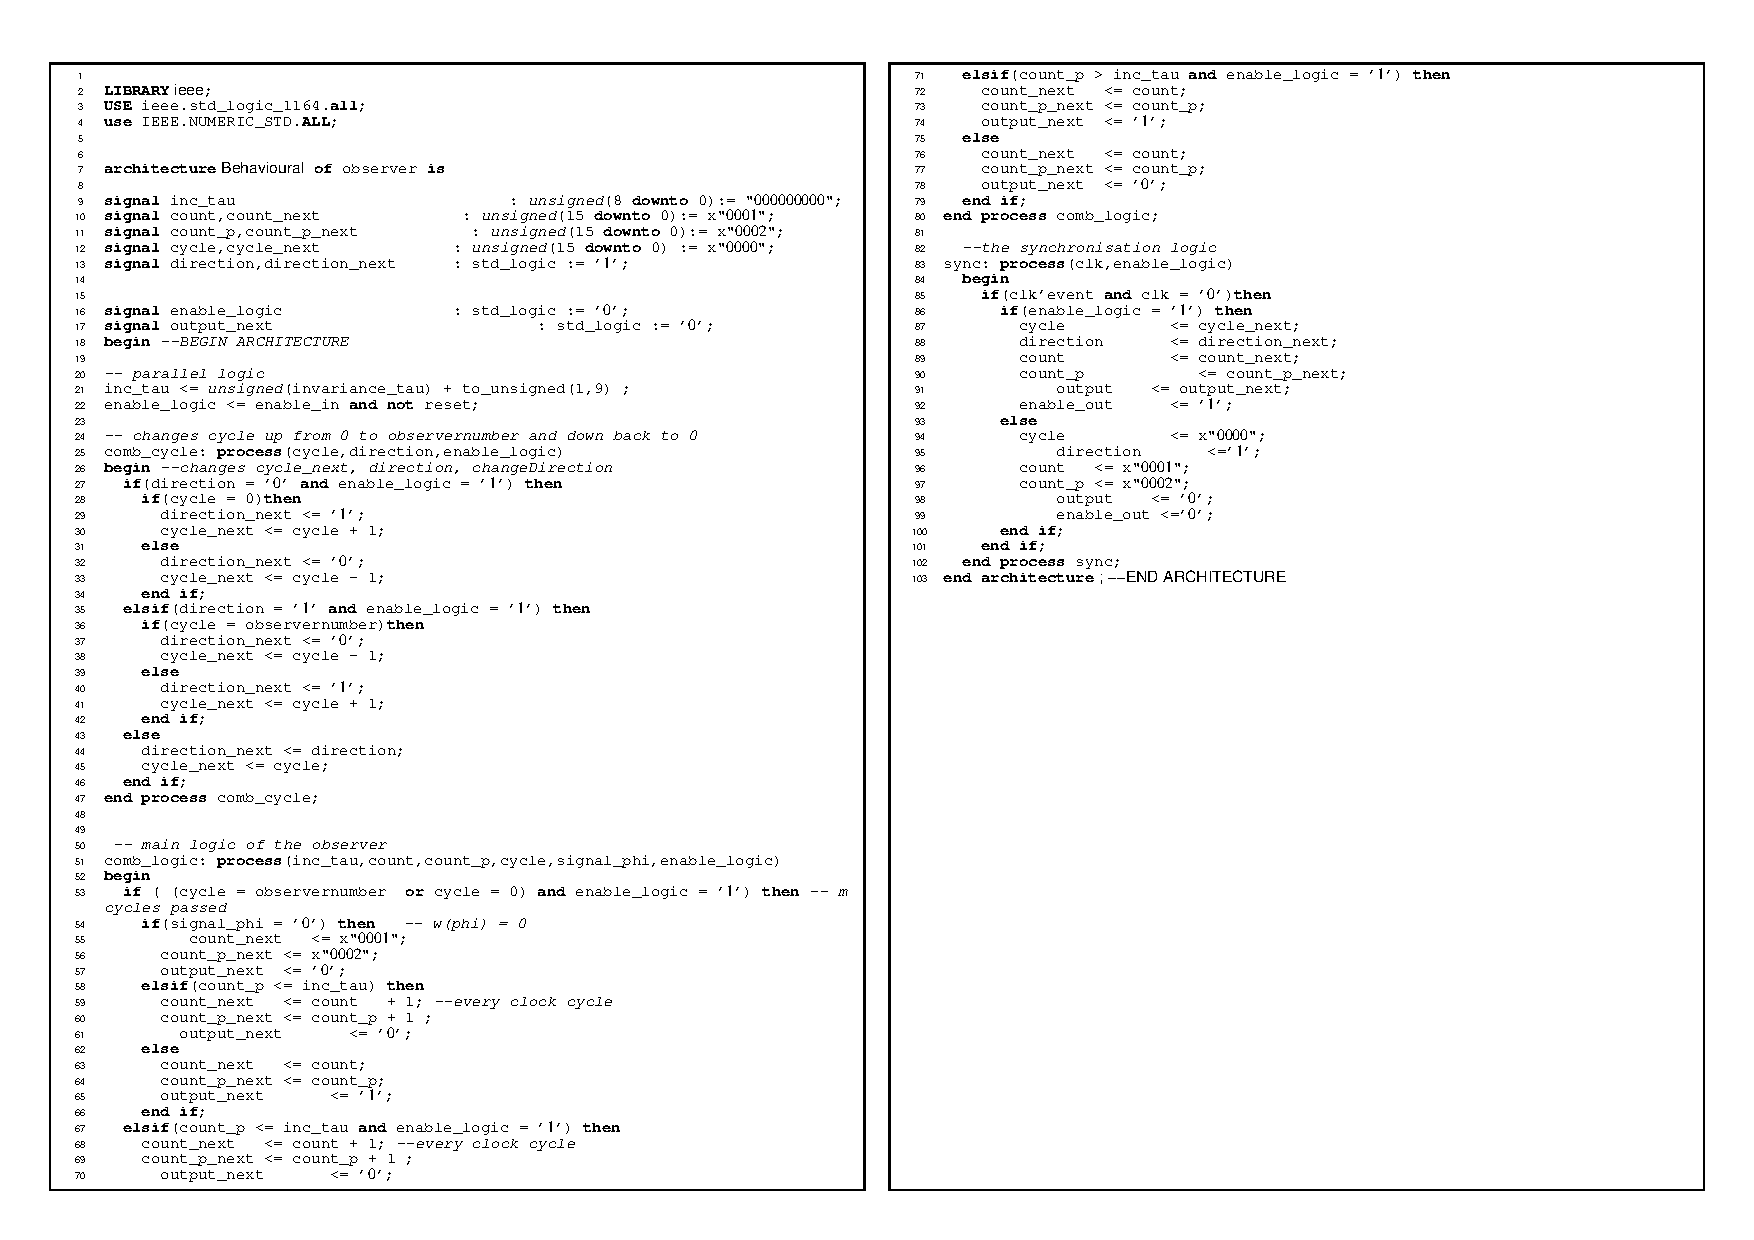
\includepdf[
 pages={-},
 nup=1x1,
 landscape=true,
 %fitpaper=true,
 noautoscale=false,
 turn=false,
 scale=0.9,
 %trim= 0mm 0mm 0mm 0mm,
 clip=true,
 %pagecommand={\label{appendix:source:2}},
 pagecommand={},
 %delta=0mm 0mm
 %offset=-80mm 0mm
 %addtotoc={1,figure,1,{Behavioural Design of Invariant Observer},{appendix:source:2}}
]{Appendix1/pdf/Observer_behave_2.pdf}
%\caption[Behavioural Design of Invariant Observer]{Code of the Behavioural Design of the Invariant Observer }
%\label{appendix:source:2}
\end{comment}

\section{Observer Stage}

\label{appendix:1:section:1}
%\section{Entity Design}
\begin{center}
\begin{figure}[]
\centering
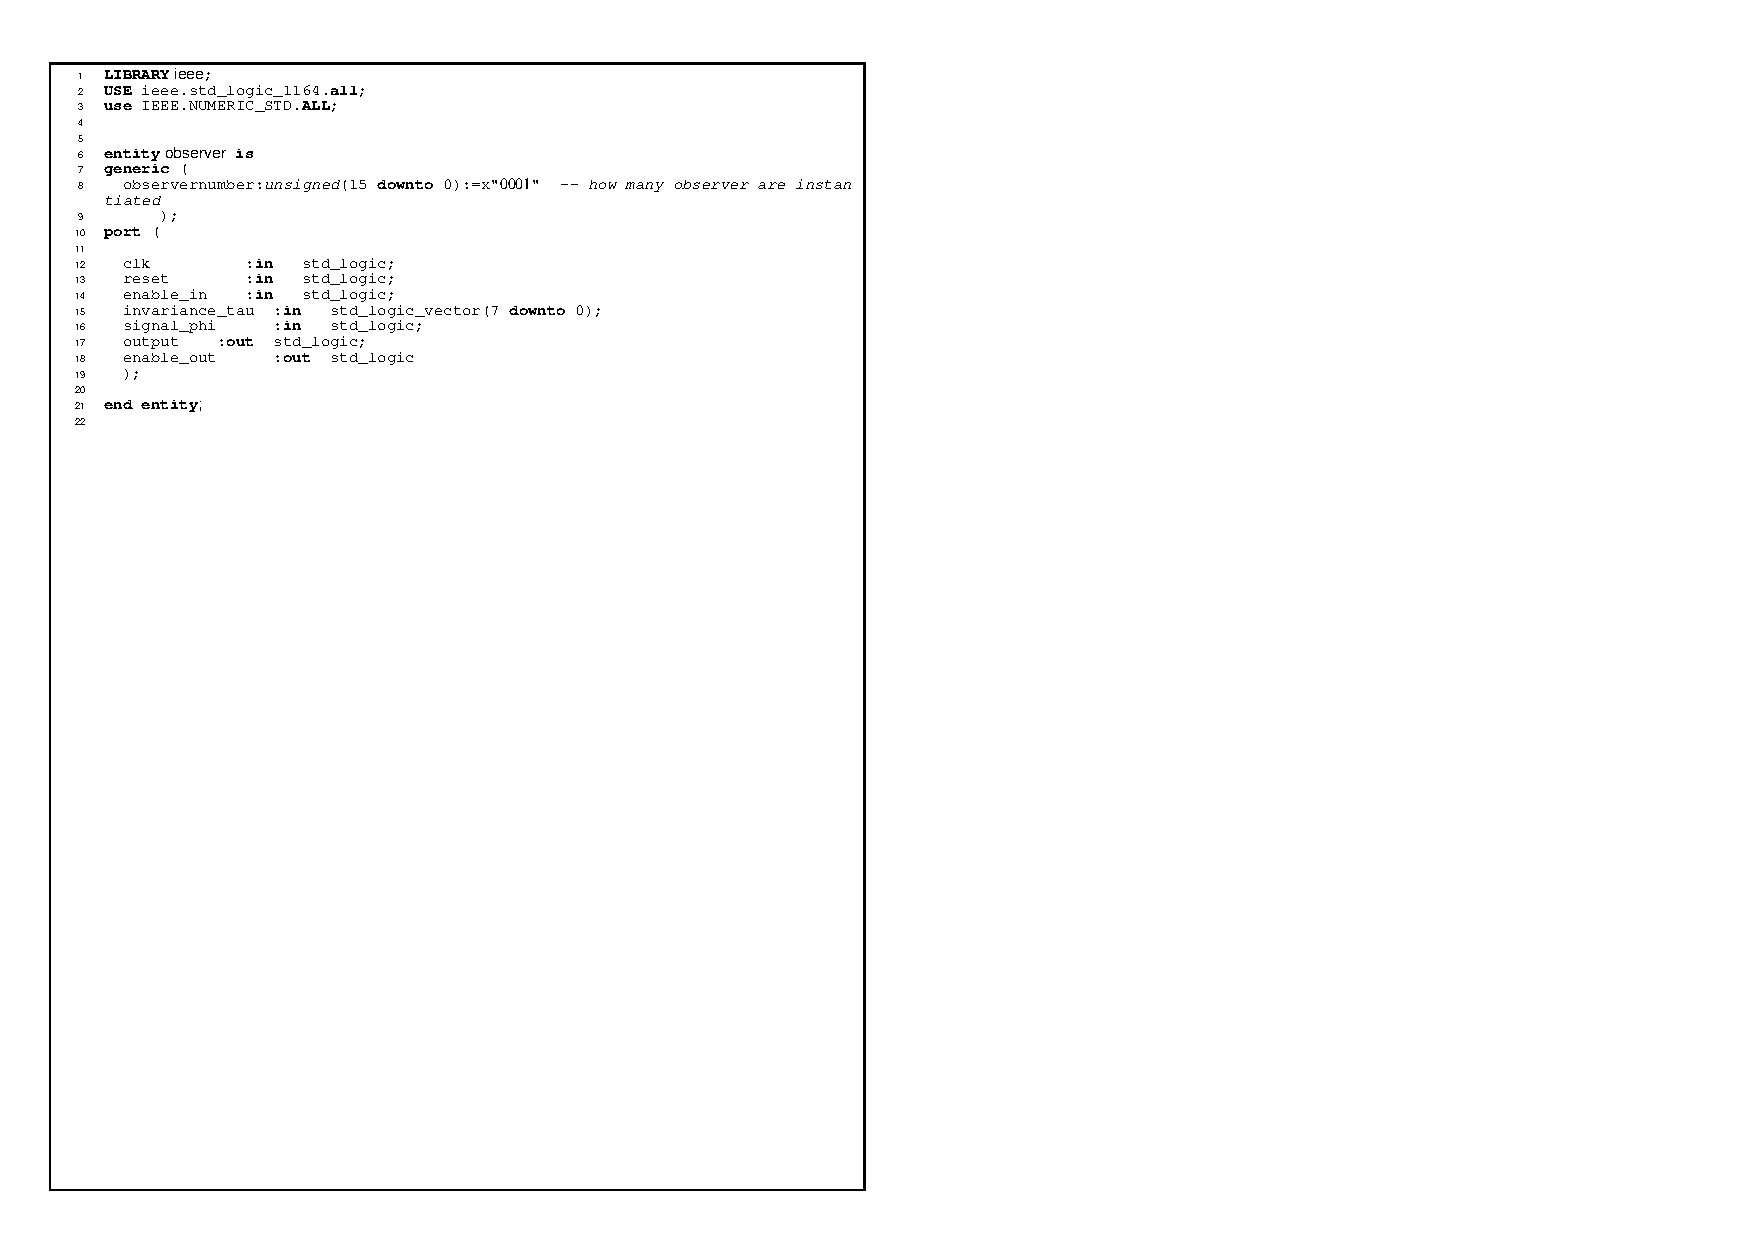
\includegraphics[scale=1.00]{Appendix1/pdf/Observer_2.pdf}
\caption[Entity Design of Invariant Observer]{Code of Observer Entity Design}
\label{appendix:source:1}
\end{figure}
\end{center}

%\section{Behavioural Design}
\begin{center}
\begin{figure}[]
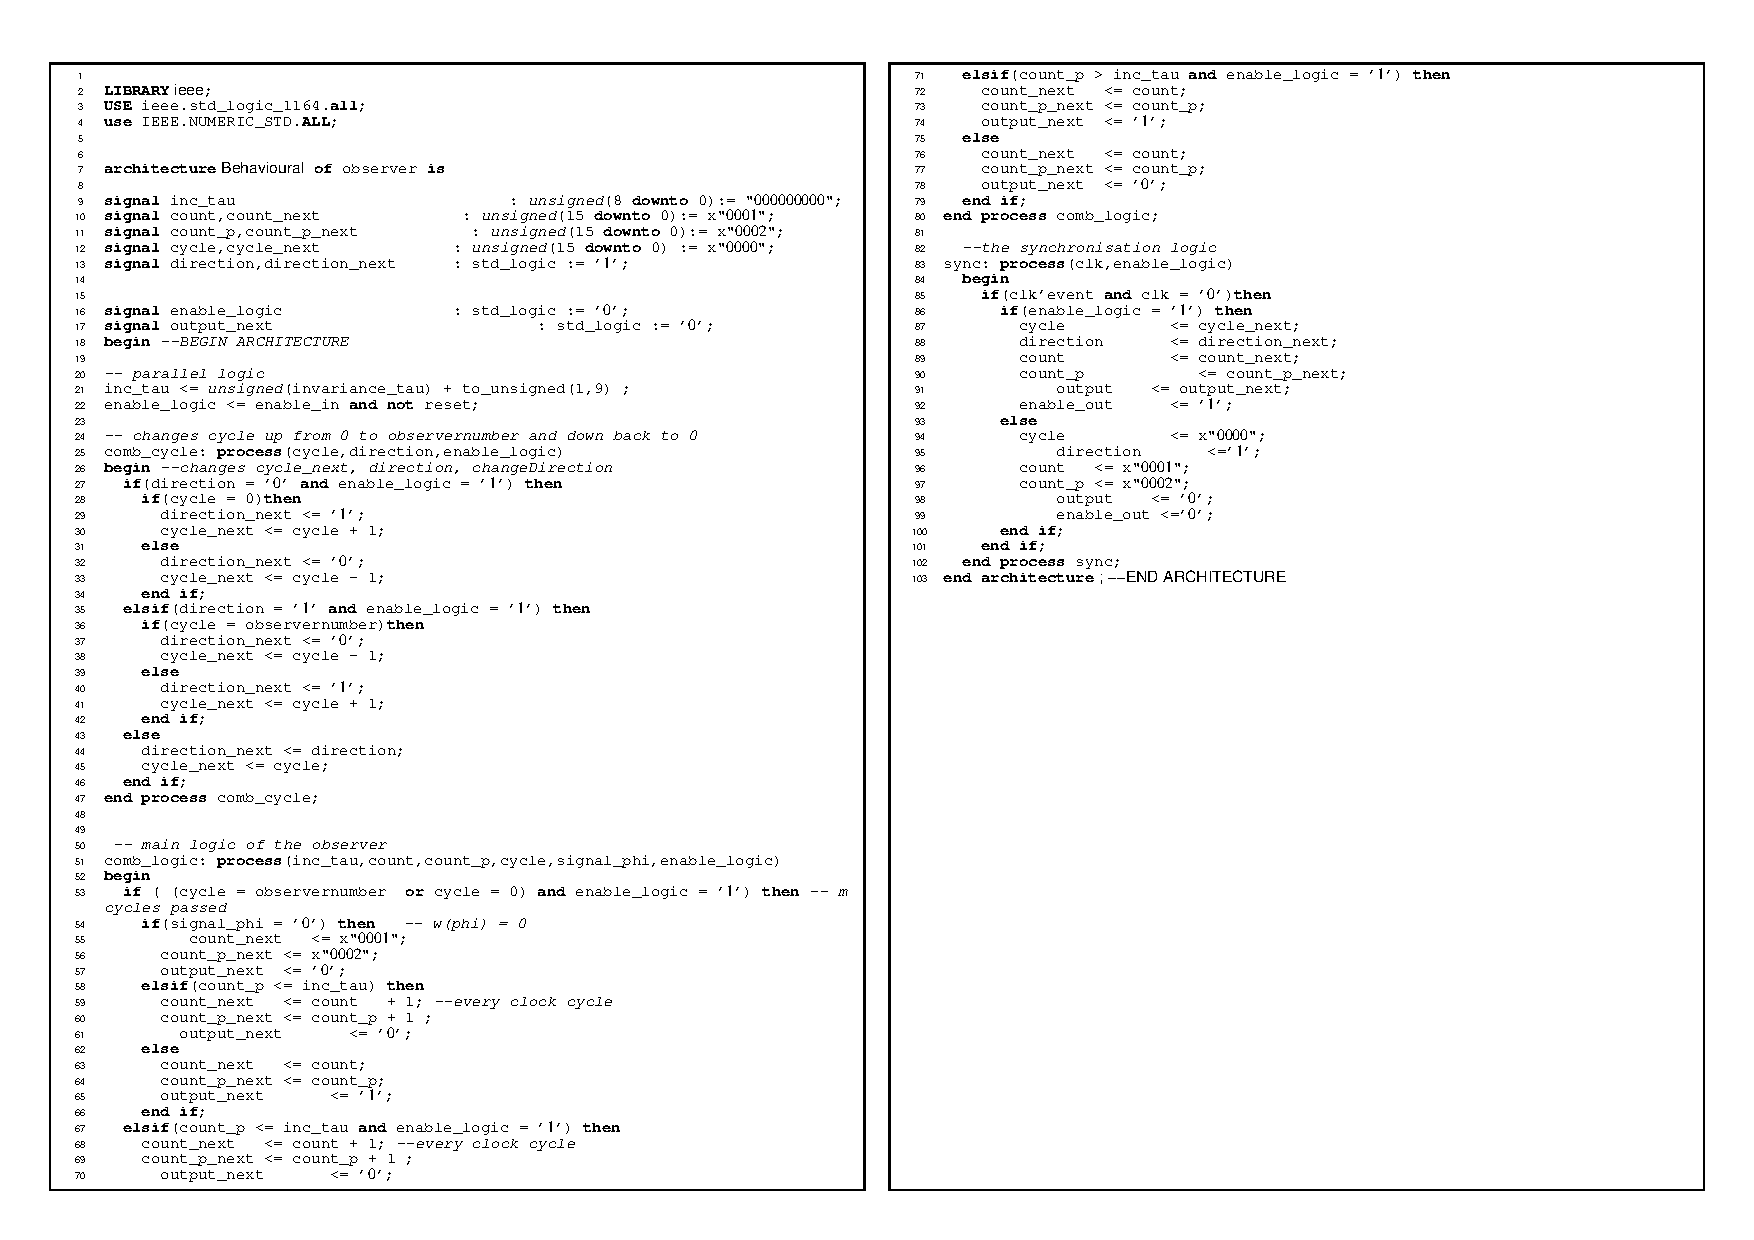
\includegraphics[scale=0.80,angle=90]{Appendix1/pdf/Observer_behave_2.pdf}
\caption[Behavioural Design of Invariant Observer]{Code of the Behavioural Design of an Invariant Observer }
\label{appendix:source:2}
\end{figure}
\end{center}

\clearpage

\section{TOP File}
\label{appendix:1:section:2}



\begin{figure}[]
\centering
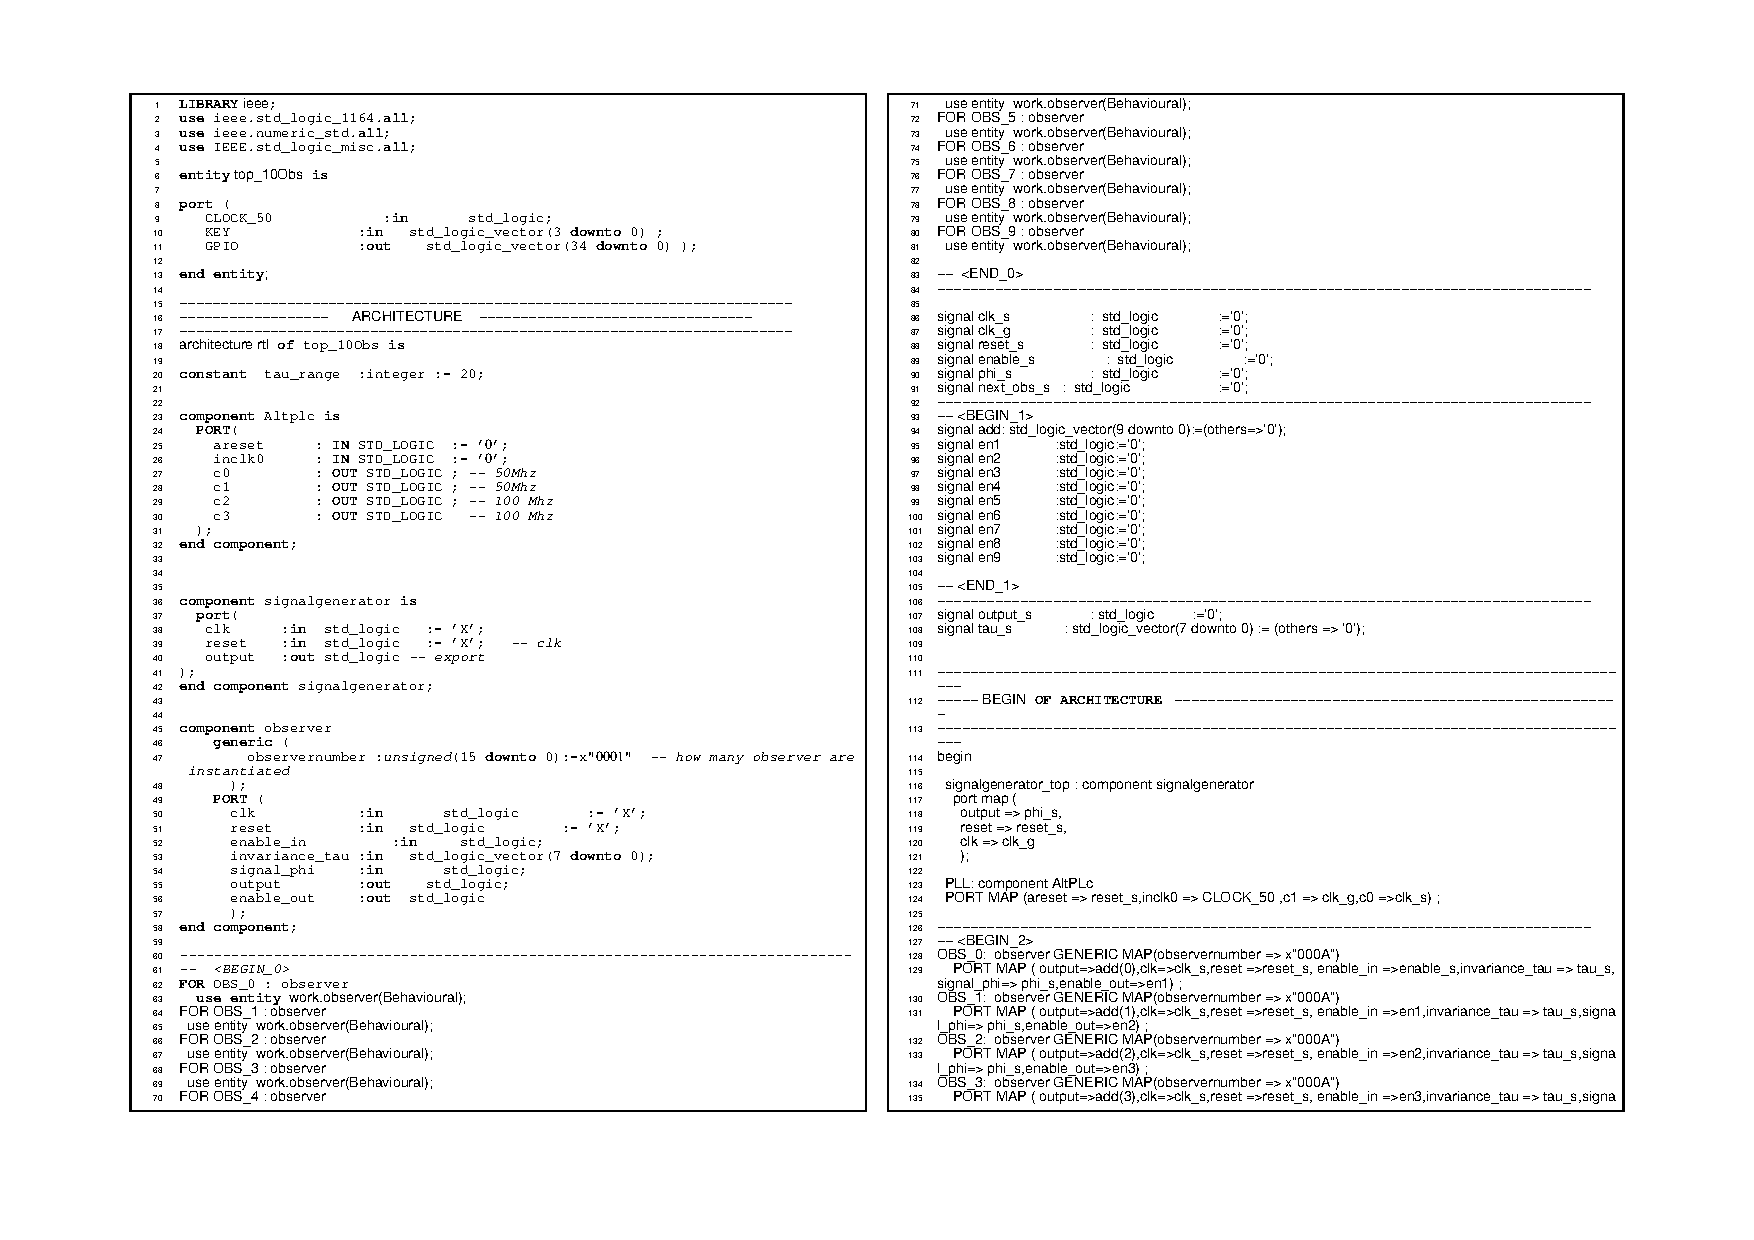
\includegraphics[scale=0.80,angle=90]{Appendix1/pdf/TOP_10OBS_1.pdf}
\caption[TOP File Example-p1]{Example Code of a TOP file for experiments}
\label{appendix:source:3}
\end{figure}


\begin{figure}[]
\centering
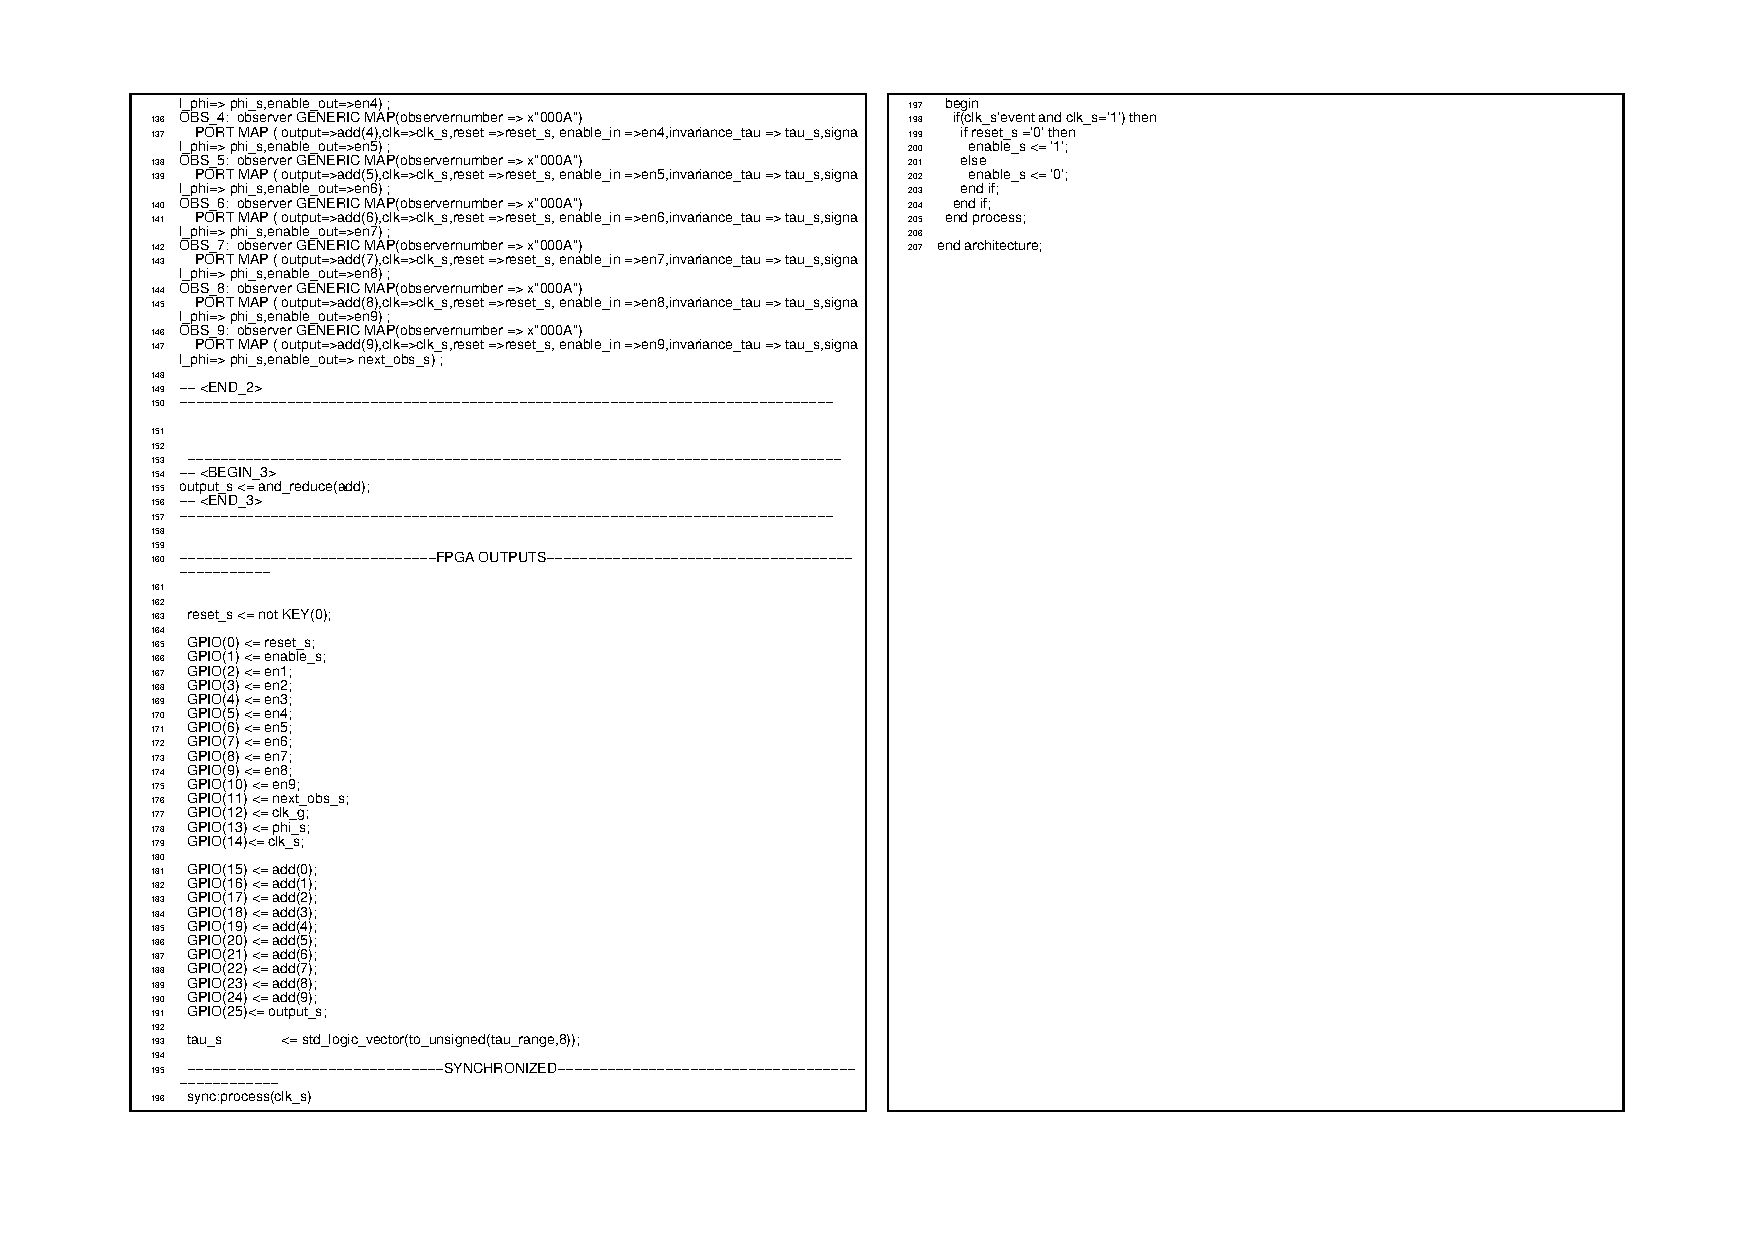
\includegraphics[scale=0.80,angle=90]{Appendix1/pdf/TOP_10OBS_2.pdf}
\caption[TOP File Example-p1]{Example Code of a TOP file for experiments}
\label{appendix:source:4}
\end{figure}












